\chapter{Bill of Materials}

\section{Overview}

As mentioned previously, Cooper Union Machine Co's Tube Notcher was designed to be cheaper than tube notchers currently on the market. To do so the machine was compared to Baleigh Industrial's Tube Notcher; the TN-800. Baileigh Industrial's design, shown below, can be purchased for \$7,995.00.

\begin{figure}[hbp]
    \centering
    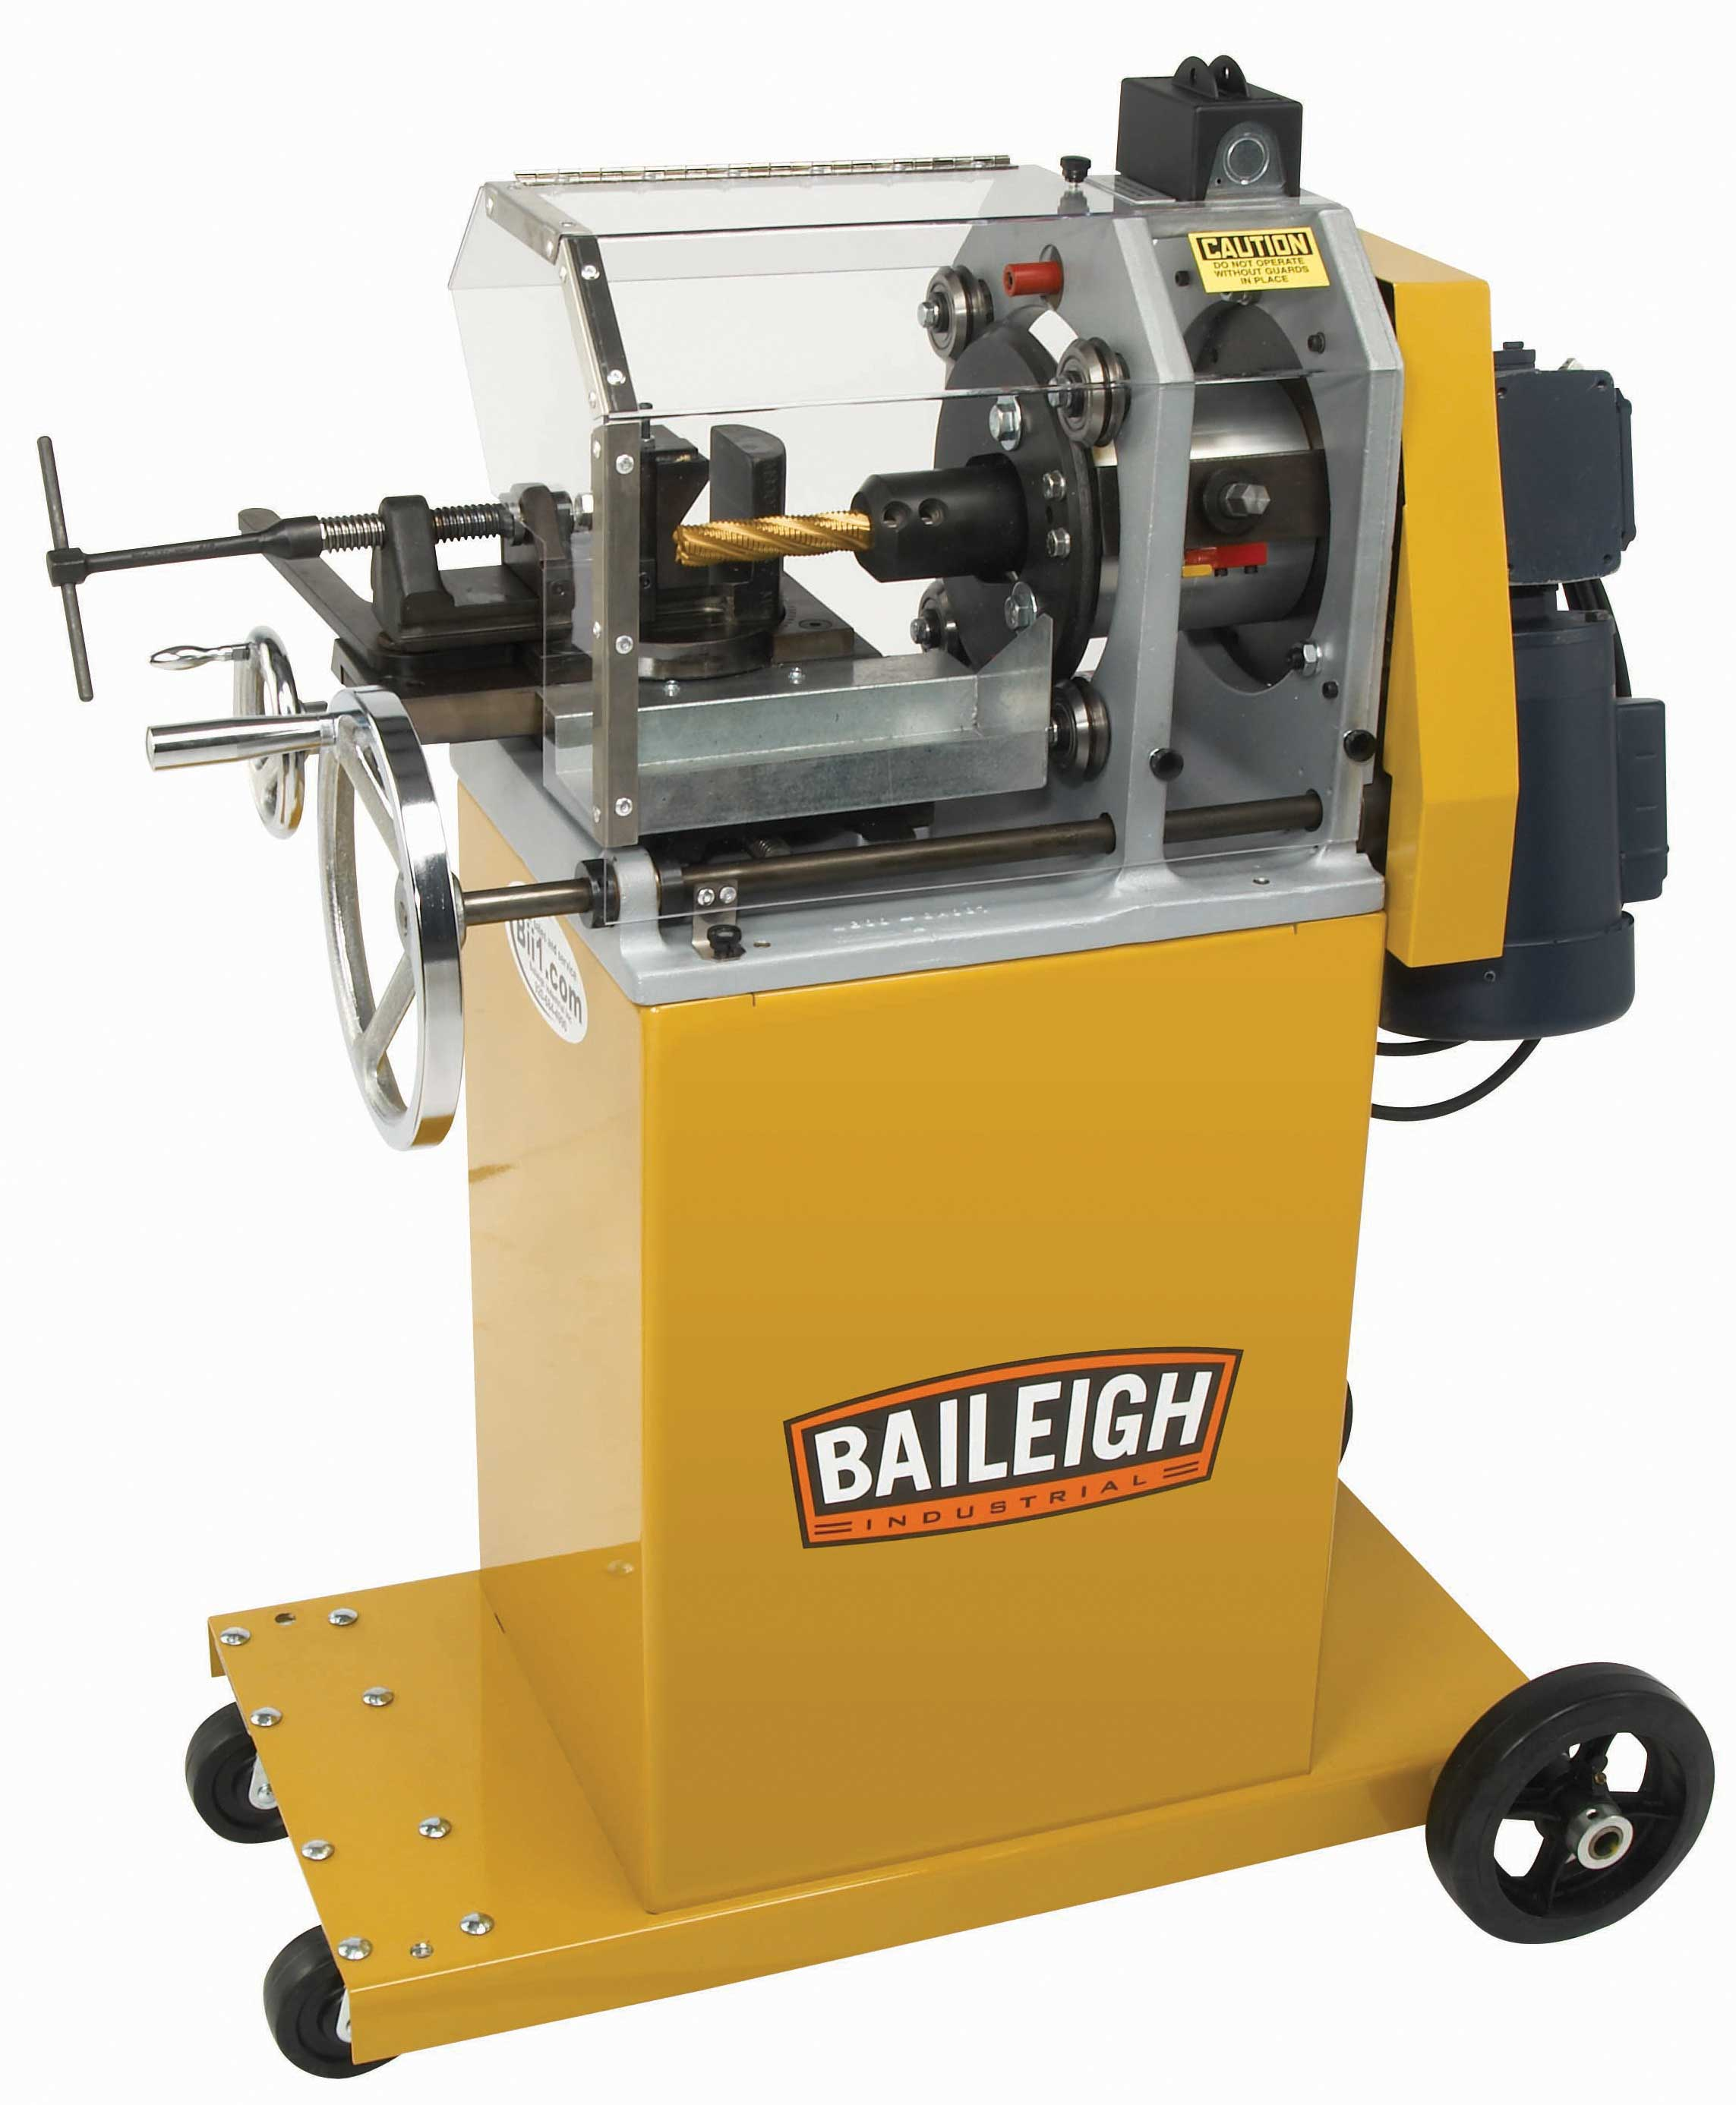
\includegraphics[width=0.4\textwidth]{./fall-report pictures/Chapter4-BillofMaterials/TN-800}
    \caption{Baileigh Industrial's TN-800 Tube and Pipe Notcher}
    \label{fig:Baileigh Industrial}
\end{figure}

After designing the machine as seen in Chapter 2, Cooper Union Machine Co's Tube Notcher costs \$3423.44 to manufacture. The cost of the Notchmatic considers two situations. The first is the full cost of the machine assuming that new materials are purchased and the entire material is built from scratch. The second is the final cost of the machine and only considers the cost of the machine to the Department of Mechanical Engineering at The Cooper Union. This removes any hardware which will be graciously provided by the Cooper Union's Machine Shop as well as all materials that were donated to the project or recycled from The Cooper Union. In reality, many of the parts were acquired from The Cooper Union. The full cost for the Notchmatic amounts to \$3000.00. After reductions, however, the final cost of the tube notcher is only \$2149.51 total. Compared to Baileigh Industrial's machine, Cooper Union Machine Co can build an equivalent system for 33\% of the cost. 

The following section lists the components and associated costs of each subsystem of the Tube Notcher.

\begin{figure}[H]
    \centering
    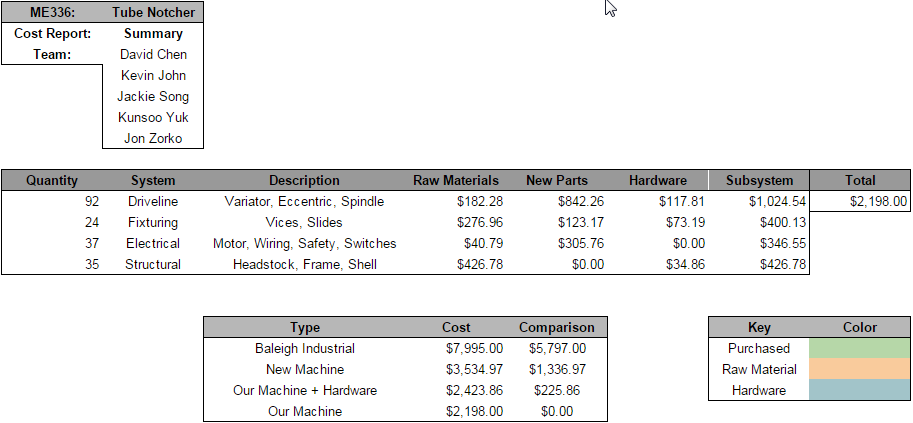
\includegraphics[width=1.0\textwidth]{./fall-report pictures/Chapter4-BillofMaterials/Overall}
    \caption{Overall Cost for CMC's Notchmatic}
    \label{fig:Overall}
\end{figure}

%------------------------------------------------------------------------------------------------------------------------------------------------------------------------------------------
\newpage

\subsection{Structural}

\begin{figure}[H]
    \centering
    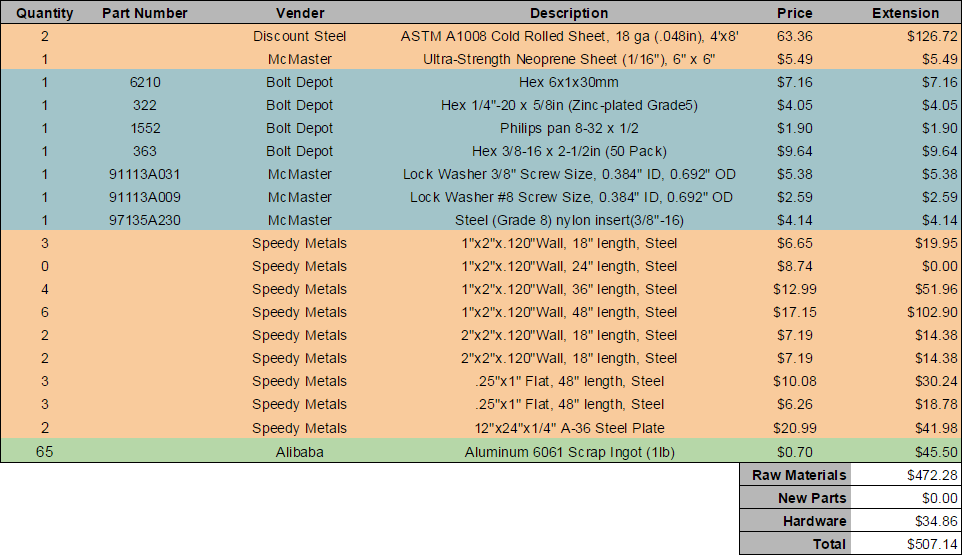
\includegraphics[width=1.0\textwidth]{./fall-report pictures/Chapter4-BillofMaterials/CRS}
    \caption{Full Cost Report for the Structural System}
    \label{fig:CRS}
\end{figure}

The structure of the Notchmatic, in total, costs \$461.64. Because the frame was designed around the loads generated by this particular machine, it was custom made. Therefore, the structure is made from only raw materials and hardware for fastening. The majority of the cost for this system comes from the raw materials which includes the steel beams for the frame, the steel sheets for the shell, and the aluminum material needed to cast the headstock. Since the maufacturing of the Notchmatic is done in-house, there is no associated manufacturing cost for the machine. Additionally, raw materials can be ordered from bulk metal suppliers as seen in  the cost report above. Suppliers such as McMaster, Bolt Depot, and Speedy Metals. The steel bed and shell material choice reduced the cost of the machine. By reinforcing the bed rather than simply using a thicker bed, the cost was reduced without jeopardizing the structural strength of the machine. Secondly, the shell cost was reduced by switching from aluminum to steel. After removing the fasteners , which will be provided by The Cooper Union Machine Shop, the final cost for the structural system reduces to \$426.78. This saves a total of \$50.00 from the overall cost of the machine. Another key cost reduction is the headstock casting material. The aluminum used to cast the headstock will come from recycled aluminum found in The Cooper Union and are ,therefore, not included in the final cost for the machine. The cost report below shows the final cost of the machine after removing the fasteners and casting material from the full cost report. This is the amount needed to build and assemble the structure for the Notchmatic at The Cooper Union.

\begin{figure}[htp]
    \centering
    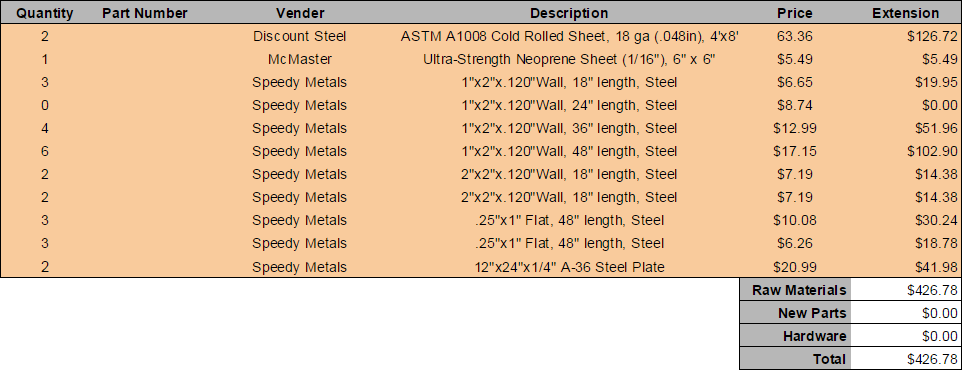
\includegraphics[width=1.0\textwidth]{./fall-report pictures/Chapter4-BillofMaterials/FCRS}
    \caption{Final Cost Report for the Structural System}
    \label{fig:FCRS}
\end{figure}


%------------------------------------------------------------------------------------------------------------------------------------------------------------------------------------------
\newpage

\subsection{Driveline}

\begin{figure}[H]
    \centering
    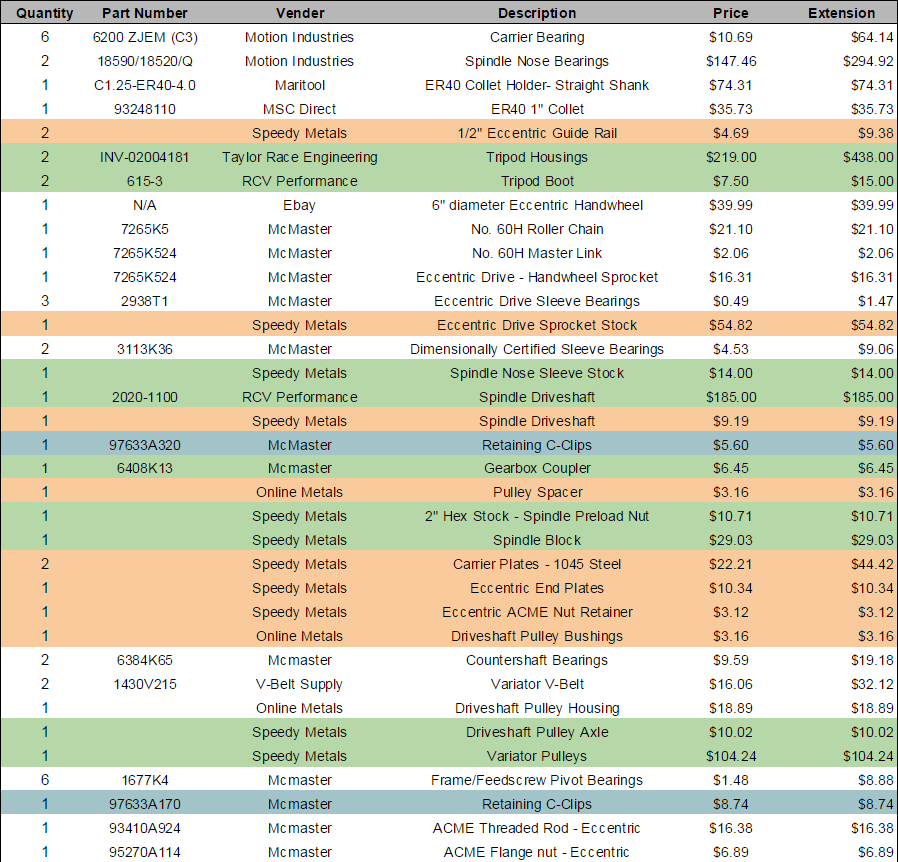
\includegraphics[width=1.0\textwidth]{./fall-report pictures/Chapter4-BillofMaterials/CRD1}
    \caption{Full Cost Report for the Driveline}
    \label{fig:CRD}
\end{figure}
\begin{figure}[H]
    \centering
    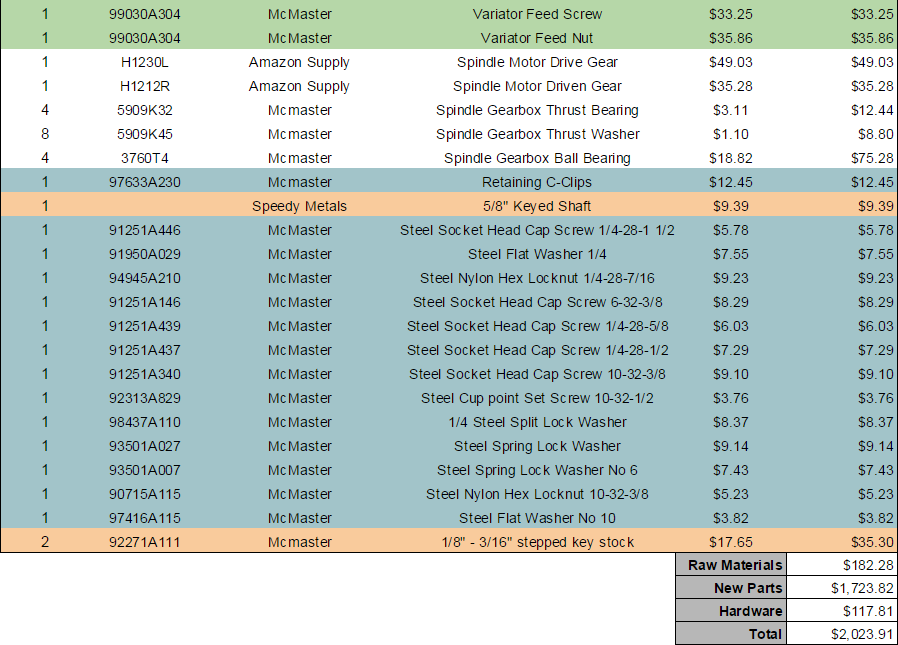
\includegraphics[width=1.0\textwidth]{./fall-report pictures/Chapter4-BillofMaterials/CRD2}
    \caption{Full Cost Report for the Driveline}
    \label{fig:CRD}
\end{figure}

Within the driveline subsystem there were two primary areas of notable cost savings. One area is the eccentric power transmission system, more specifically the CV joints, tripods, and mid-shaft. By using old Formula SAE spec. components, not only is approximately \$500 saved, but also the components are oversized by a factor of four. The other notable area of cost savings is the spindle nose bearings. Traditionally, ABEC -7 machine-grade bearings are used to meet the demands of the high speed, high load conditions of the spindle nose. Bearings of this precision rating often cost around \$1300 each.  The more economical approach is to use bearings with a lower precision rating. However, simply using bearings with a lower precision rating will negatively impact the overall precision attainable with the machine. To offset this, a preloading torque is placed on these bearings. This preloading torque forces the concentricity of the spindle bearings to increase. This technique made it possible to use a set of ABEC-3 tapered roller bearings which cost \$150 each. 

\begin{figure}[htp]
    \centering
    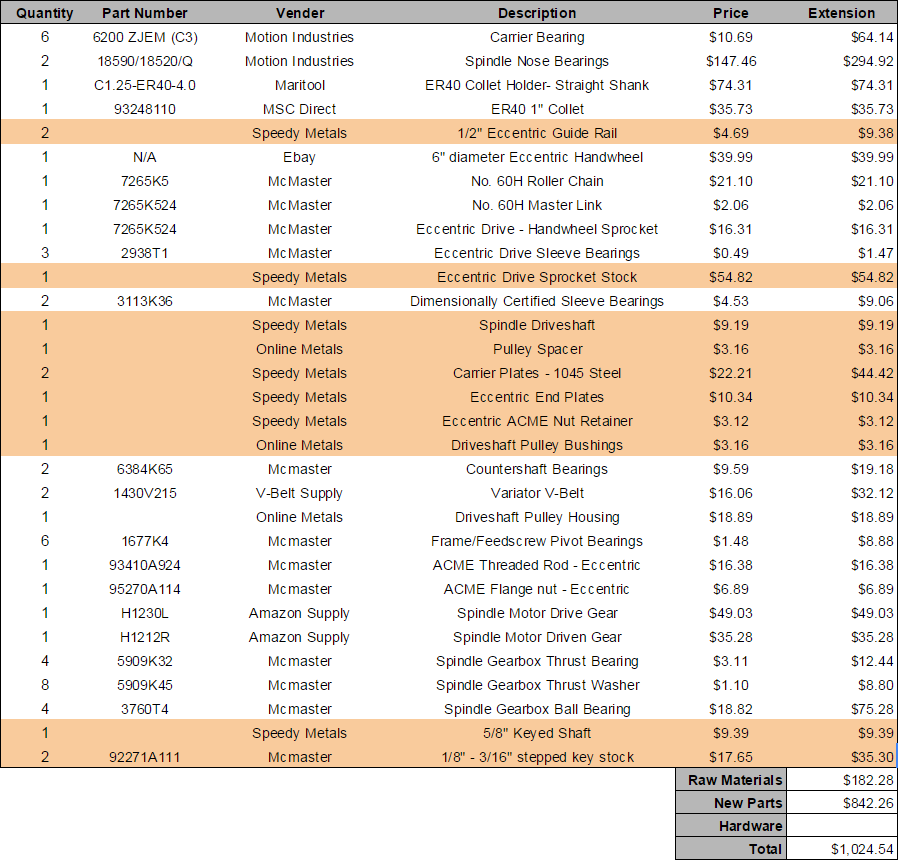
\includegraphics[width=1.0\textwidth]{./fall-report pictures/Chapter4-BillofMaterials/FCRD}
    \caption{Final Cost Report for the Driveline}
    \label{fig:CRD}
\end{figure}


%------------------------------------------------------------------------------------------------------------------------------------------------------------------------------------------
\newpage

\subsection{Fixturing}

\begin{figure}[H]
    \centering
    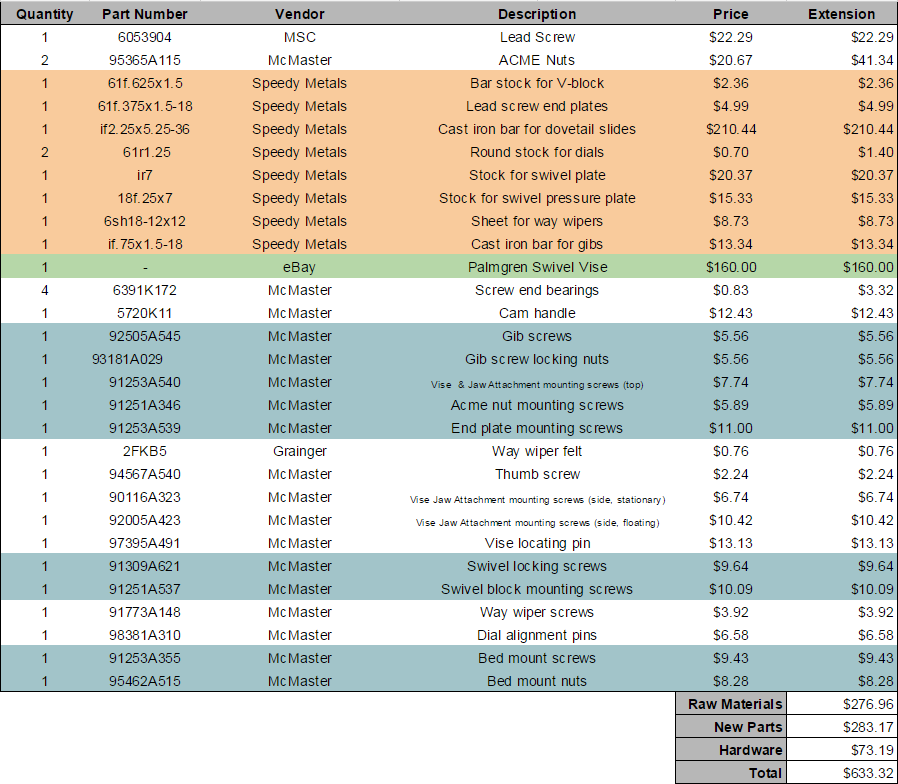
\includegraphics[width=1.0\textwidth]{./fall-report pictures/Chapter4-BillofMaterials/CRF}
    \caption{Full Cost Report for the Fixturing Mechanism}
    \label{fig:CRD}
\end{figure}

The fixturing mechanism of the Notchmatic, in total, costs \$633.32. As shown in the full cost report, the fixturing requires raw materials, fasteners, and new parts. Larger parts of the fixturing such as the dovetail stages, lead screws, rotational plates, and vblock are made from raw materials. Costs were reduced by buying larger blocks and machining them down as opposed to buying many smaller blocks. The greatest cost reduction in the design was achieved by removing the vice from the cost report. A vice was graciously donated to The Cooper Union Machine Co. by Professor Estuardo Rodas thereby reducing the cost by \$160.00. Since the fixturing mechansim bears the majority of the cutting forces during the machine's operations, the quality and strength of this subsystem could not be jeopordized. Specific fastening equipment is also needed for this same reason. After removing the vice and the fasteners from the cost report, the final cost of the fixturing mechanisms is \$400.13. The final budget for the fixturing mechanism is reduced to 63.2\% of it's original full cost.  

\begin{figure}[htp]
    \centering
    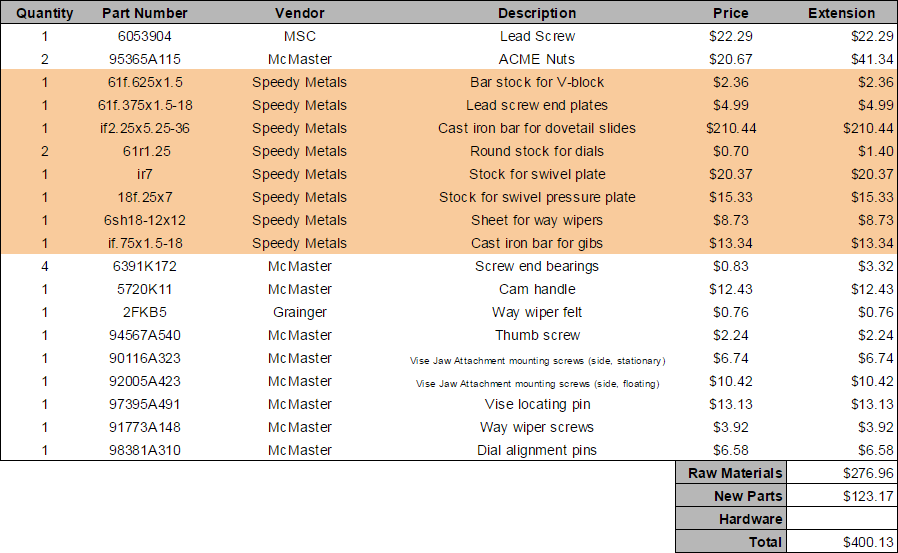
\includegraphics[width=1.0\textwidth]{./fall-report pictures/Chapter4-BillofMaterials/FCRF}
    \caption{Final Cost Report for the Fixturing Mechanism}
    \label{fig:FCRF}
\end{figure}


%------------------------------------------------------------------------------------------------------------------------------------------------------------------------------------------
\newpage

\subsection{Electrical}

\begin{figure}[H]
    \centering
    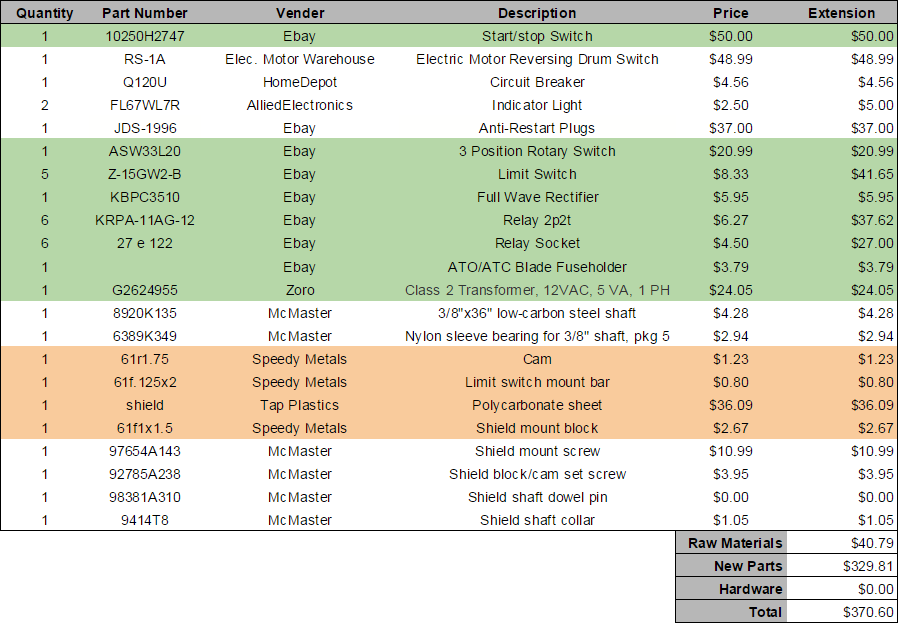
\includegraphics[width=1.0\textwidth]{./fall-report pictures/Chapter4-BillofMaterials/CRE}
    \caption{Full Cost Report for the Electrical System}
    \label{fig:CRE}
\end{figure}

The electrical system of the Notchmatic, in total, costs \$370.60. The larget portion of the budget of the cost for the electronics of the Notchmatic comes from the switches that allow the machine to function. All seven switches were purchased for \$161.63. The remaining 56.4\% of the electrical system budget is composed of electrical components and raw materials for the safety shield. Raw materials for the control box and control panel will come from left over material from the structural and driveline systems. Most of the switches used are common for industry applications and, therefore, could be purchased from 3rd party websites. Although this is already included in the full cost report, it greatly reduced the cost. Consequently, "new" switches and relays could be purchased at "used" prices from ebay. Not only did this reduce the cost but it also did so without jeopordizing the safety of the user or functionality of the machine.
Since there are no fastners included in the electronics system, cost was only reduced when a transformer was provided by Estuardo Rodas. From this reduction the final cost of the electrical system becomes \$346.55.

\begin{figure}[htp]
    \centering
    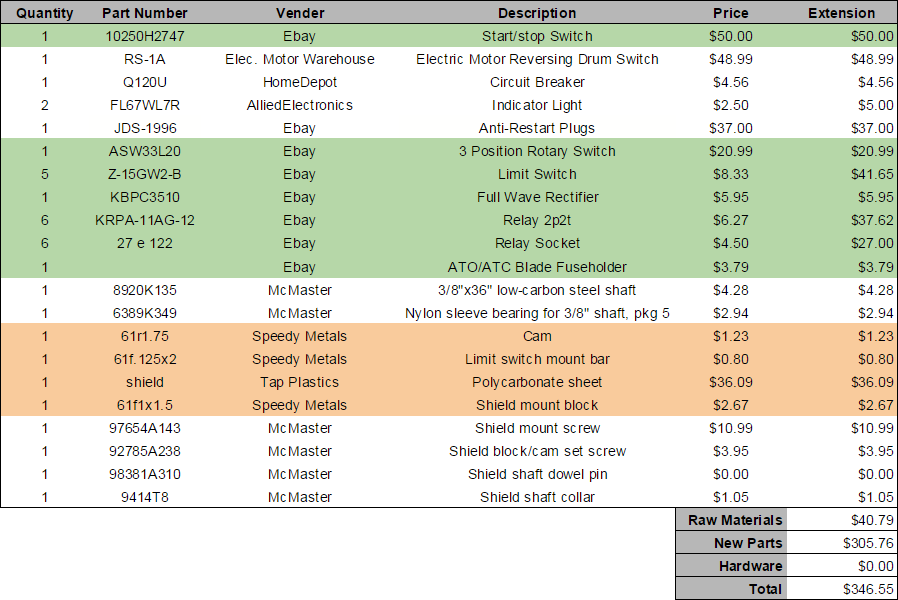
\includegraphics[width=1.0\textwidth]{./fall-report pictures/Chapter4-BillofMaterials/FCRE}
    \caption{Final Cost Report for the Electrical System}
    \label{fig:FCRE}
\end{figure}